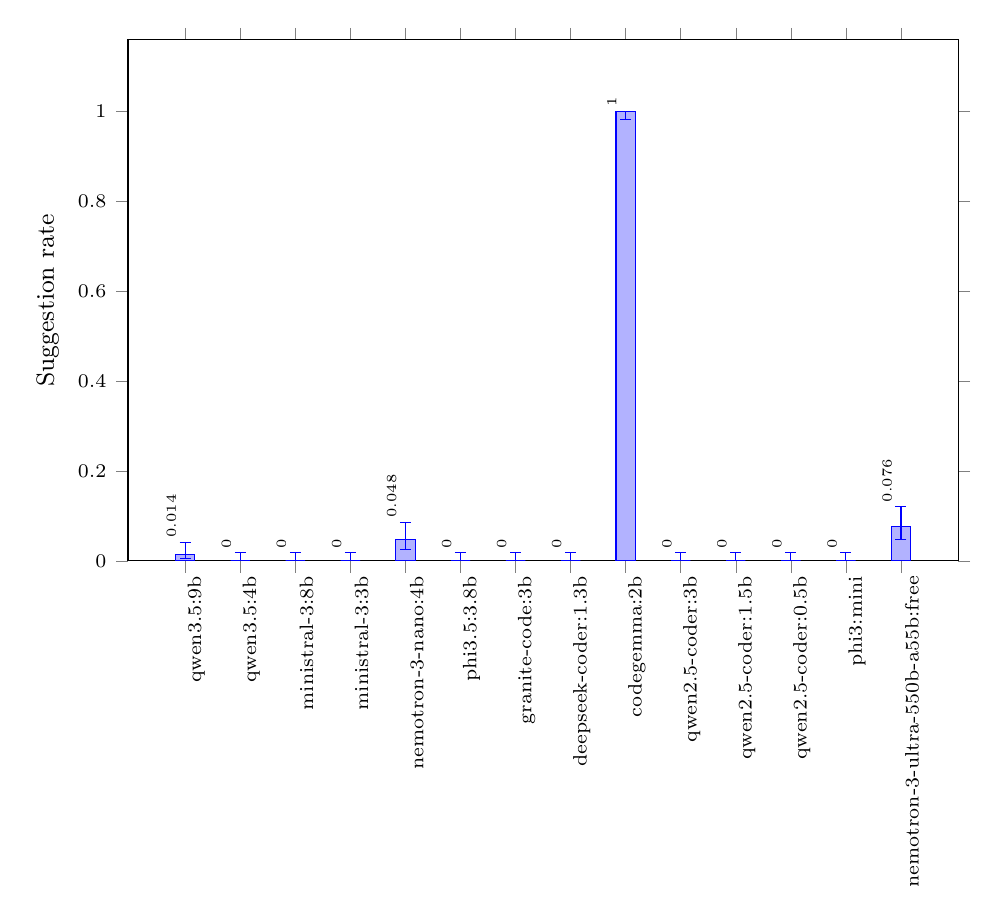
\begin{tikzpicture}
\begin{axis}[
  ybar,
  bar width=7pt,
  bar shift=0pt,
  width=\textwidth,
  height=8.2cm,
  ylabel={Suggestion rate},
  xtick={0,1,2,3,4,5,6,7,8,9,10,11,12,13},
  xticklabels={qwen3.5:9b,qwen3.5:4b,ministral-3:8b,ministral-3:3b,nemotron-3-nano:4b,phi3.5:3.8b,granite-code:3b,deepseek-coder:1.3b,codegemma:2b,qwen2.5-coder:3b,qwen2.5-coder:1.5b,qwen2.5-coder:0.5b,phi3:mini,nemotron-3-ultra-550b-a55b:free},
  x tick label style={rotate=90, anchor=east, font=\scriptsize, inner sep=1pt, yshift=-4pt},
  y tick label style={font=\scriptsize},
  label style={font=\small},
  ymin=0,
  ymax=1.160000,
  enlarge x limits=0.08,
  tick align=outside,
  clip=false,
]
\addplot+[
  bar shift=0pt,
  error bars/.cd,
  y dir=both,
  y explicit,
  error bar style={thin}
] table[x=x,y=y,y error minus=minus,y error plus=plus] {
x y minus plus
0 0.014286 0.009416 0.026866
1 0.000000 0.000000 0.017964
2 0.000000 0.000000 0.017964
3 0.000000 0.000000 0.017964
4 0.047619 0.021551 0.037804
5 0.000000 0.000000 0.017964
6 0.000000 0.000000 0.017964
7 0.000000 0.000000 0.017964
8 1.000000 0.017964 0.000000
9 0.000000 0.000000 0.017964
10 0.000000 0.000000 0.017964
11 0.000000 0.000000 0.017964
12 0.000000 0.000000 0.017964
13 0.076190 0.028751 0.043978
};
\addplot[
  only marks,
  mark=none,
  bar shift=0pt,
  forget plot,
  nodes near coords,
  point meta=explicit symbolic,
  every node near coord/.append style={font=\tiny, rotate=90, anchor=west, inner sep=1.5pt, yshift=5pt, fill=white, fill opacity=0.9, text opacity=1},
] table[x=x,y=y,meta=label] {
x y label
0 0.041152 {0.014}
1 0.017964 {0}
2 0.017964 {0}
3 0.017964 {0}
4 0.085423 {0.048}
5 0.017964 {0}
6 0.017964 {0}
7 0.017964 {0}
8 1.000000 {1}
9 0.017964 {0}
10 0.017964 {0}
11 0.017964 {0}
12 0.017964 {0}
13 0.120168 {0.076}
};
\end{axis}
\end{tikzpicture}
